 
\documentclass{article}
\usepackage[utf8]{inputenc}
\usepackage[brazil]{babel} 


\usepackage{caption} 
\usepackage{float}  
\usepackage{graphicx}   
\usepackage{subcaption}
\title{Figuras lado a lado utilizando o pacote subcaption}
\author{Rafael Soratto} 
\date{\today}   

\begin{document}

\maketitle

\section{O pacote subcaption}
\begin{figure}[H] 
\caption{Two simple graphs}
\label{fig:three graphs}
     \centering
     \begin{subfigure}[H]{0.4\textwidth}
         \centering 
         \caption{$y=3sinx$}
         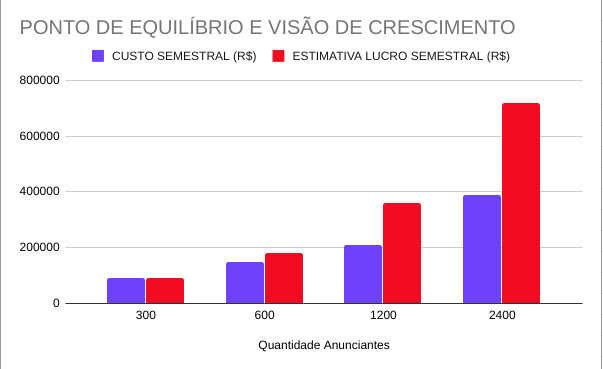
\includegraphics[width=\textwidth]{PONTOEQ}
         \label{fig:three sin x}
     \end{subfigure}
     \hfill
     \begin{subfigure}[H]{0.4\textwidth}
         \centering 
              \caption{$y=5/x$}
         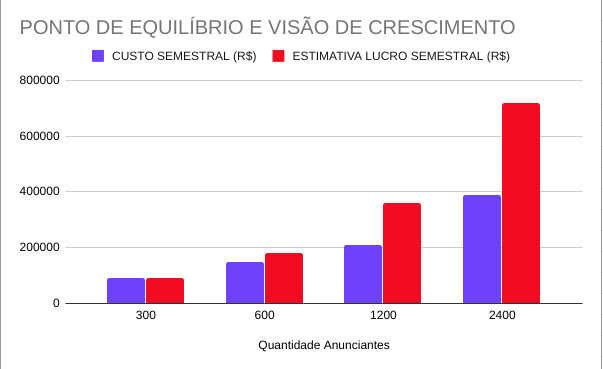
\includegraphics[width=\textwidth]{PONTOEQ.png}
         \label{fig:five over x}
     \end{subfigure} 
\leftline{  \footnotesize Fonte: autoria própria (2018).}     
\end{figure}
\begin{figure}[H] 
\caption{Two simple graphs}
\label{fig:three graphs}
     \centering
     \begin{subfigure}[H]{0.4\textwidth}
         \centering 
         \caption{$y=3sinx$}
         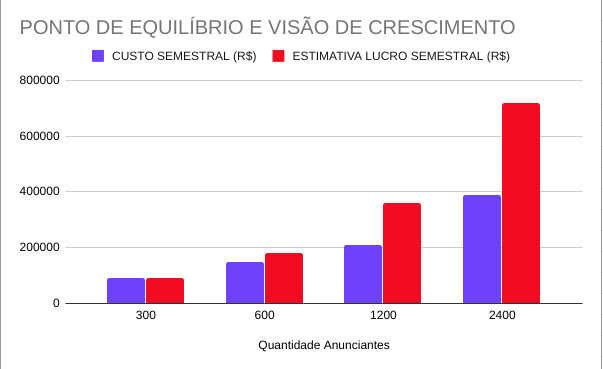
\includegraphics[width=\textwidth]{PONTOEQ}
         \label{fig:three sin x}
     \end{subfigure}
     \hfill
     \begin{subfigure}[H]{0.4\textwidth}
         \centering 
              \caption{$y=5/x$}
         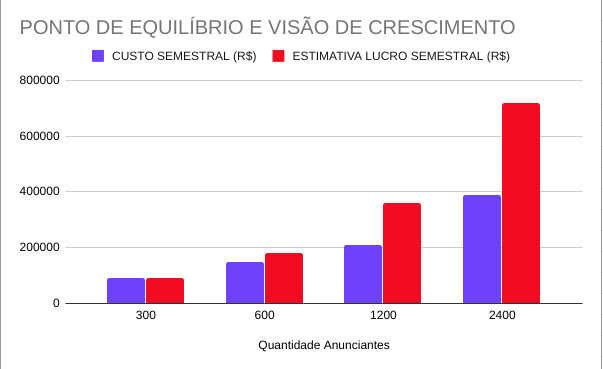
\includegraphics[width=\textwidth]{PONTOEQ}
         \label{fig:five over x}
     \end{subfigure} 
\leftline{  \footnotesize Fonte: autoria própria (2018).}     
\end{figure}

\end{document}